\documentclass[10pt]{article}
\usepackage[utf8]{inputenc}
\usepackage[T1]{fontenc}
\usepackage[margin=0.75in]{geometry}
\usepackage{amsmath,amssymb,amsthm}
\usepackage{graphicx}
\usepackage{booktabs}
\usepackage{algorithm}
\usepackage{algpseudocode}
\usepackage[table]{xcolor}
\usepackage{tikz}
\usetikzlibrary{shapes,arrows,positioning,fit,backgrounds,shadows,shadows.blur}
\usepackage{pgfplots}
\pgfplotsset{compat=1.17}
\usepackage{subcaption}
\usepackage{float}
\usepackage{multirow}
\usepackage{tcolorbox}
\usepackage{enumitem}
\usepackage{microtype}
\usepackage{titlesec}
\usepackage{tabularx}
\usepackage{array}
\usepackage{natbib}
\usepackage{url}

% Professional spacing
\setlength{\parskip}{0pt}
\setlength{\parindent}{10pt}
\setlength{\columnsep}{0.25in}

% Professional section formatting
\titleformat{\section}{\large\bfseries\sffamily}{\thesection}{0.5em}{}[\vspace{-0.5em}]
\titleformat{\subsection}{\normalsize\bfseries\sffamily}{\thesubsection}{0.5em}{}[\vspace{-0.3em}]
\titleformat{\subsubsection}{\small\bfseries\sffamily}{\thesubsubsection}{0.5em}{}

% Figma-inspired color palette
\definecolor{figmapurple}{RGB}{151,71,255}
\definecolor{figmablue}{RGB}{0,114,255}
\definecolor{figmateal}{RGB}{14,178,178}
\definecolor{figmagreen}{RGB}{0,200,117}
\definecolor{figmaorange}{RGB}{255,123,0}
\definecolor{figmared}{RGB}{255,59,92}
\definecolor{figmapink}{RGB}{255,99,205}
\definecolor{figmayellow}{RGB}{255,198,0}

% UI colors
\definecolor{figmabg}{RGB}{249,250,251}
\definecolor{figmatext}{RGB}{31,35,40}
\definecolor{figmagray}{RGB}{196,201,208}
\definecolor{figmalightgray}{RGB}{243,244,246}

% Legacy color names
\definecolor{accentblue}{RGB}{0,114,255}
\definecolor{darkgray}{RGB}{31,35,40}
\definecolor{darkblue}{RGB}{0,91,204}
\definecolor{lightgray}{RGB}{249,250,251}
\definecolor{alertred}{RGB}{255,59,92}
\definecolor{rowgray}{RGB}{249,250,251}
\definecolor{rowhighlight}{RGB}{232,240,254}
\definecolor{lightgreen}{RGB}{220,252,231}
\definecolor{lightyellow}{RGB}{255,251,230}

% Result boxes
\newtcolorbox{resultbox}[1][]{
  colback=lightgray,
  colframe=darkgray,
  boxrule=0.5pt,
  arc=2pt,
  left=8pt,
  right=8pt,
  top=6pt,
  bottom=6pt,
  fontupper=\small\sffamily,
  #1
}

% Hyperlinks
\usepackage[colorlinks=true,linkcolor=accentblue,citecolor=darkgray,urlcolor=accentblue]{hyperref}

% Custom commands
\newcommand{\E}{\mathbb{E}}
\newcommand{\R}{\mathbb{R}}
\newcommand{\vq}{\mathbf{q}}
\newcommand{\vk}{\mathbf{k}}
\newcommand{\vv}{\mathbf{v}}
\newcommand{\vu}{\mathbf{u}}

% Theorem environments
\newtheorem{theorem}{Theorem}
\newtheorem{proposition}{Proposition}
\newtheorem{definition}{Definition}
\newtheorem{corollary}{Corollary}
\newtheorem{observation}{Observation}

% Title and authors
\title{\vspace{-2em}\textbf{\Large The COFFEE Law: Empirical Evidence for\\Ornstein-Uhlenbeck Dynamics in LLM Context\vspace{-0.5em}}}

\author{
Manish Bhatt\\
\texttt{manish.bhatt13212@gmail.com}
}


\date{\vspace{-1em}}

\begin{document}

\maketitle

\begin{abstract}
\noindent We present empirical evidence that output embedding dynamics in transformer language models follow Ornstein-Uhlenbeck (OU) rather than Brownian motion. Our key finding is \textit{bidirectional convergence}: same-prompt continuations diverge then saturate, while cross-prompt embeddings converge then plateau. Both directions settling to equilibrium is the defining signature of mean-reverting OU processes.

Using dense hierarchical sampling (33 positions, 50 prompts, 10 domains), we validate three OU properties: (1) variance saturation at $\sigma^2_\infty \approx 0.109$ ($R^2 = 0.67$); (2) relaxation time $\tau \approx 10.6$ tokens; and (3) cross-prompt mean-reversion with Hurst exponent $H = -0.03$ ($R^2 = 0.84$). We replicate the Liu et al. ``Lost in the Middle'' U-curve (87\% edge vs 73\% middle accuracy, $n=525$), connecting it to OU saturation dynamics. Results hold across temperatures, domains, and model pairs.

We term this the \textbf{COFFEE Law}: \textbf{C}ontext-\textbf{O}ptimized \textbf{F}low with \textbf{F}ast \textbf{E}xponential \textbf{E}quilibrium. If context dynamics are mean-reverting rather than diffusive, ``long-context pessimism'' heuristics are miscalibrated. Context engineering shifts from ``prevent drift'' to ``manage the transient'': align chunk sizes and memory weights to the equilibration scale ($\sim$95\% saturation by $3\tau \approx 32$ tokens).
\end{abstract}

\noindent\textbf{\small Keywords:} Embedding Dynamics, Variance Saturation, Ornstein-Uhlenbeck Process, Context Engineering, Large Language Models

\vspace{0.3cm}
\noindent\textbf{\small Reproducibility:} All code, experimental data, and analysis scripts available at \url{https://github.com/mbhatt1/coffee-law}

\section{Introduction}

Understanding how model representations evolve during generation is critical for retrieval-augmented generation (RAG), multi-turn dialogue, and long-context applications. A common implicit assumption---which we term the \textit{Query Drift Hypothesis}---models internal query evolution as Brownian motion, predicting unbounded variance growth and progressive information loss. This assumption underlies pessimistic heuristics about context degradation \citep{liu2023lost}.

We present empirical evidence that output embedding dynamics instead follow an Ornstein-Uhlenbeck (OU) process---a mean-reverting stochastic model where variance saturates rather than growing unboundedly. Our key finding is \textit{bidirectional convergence}: same-prompt continuations diverge then saturate, while cross-prompt embeddings converge then plateau. Both directions settling to equilibrium is the hallmark of OU mean-reversion. We validate all three OU properties and term this the \textbf{COFFEE Law}: \textbf{C}ontext-\textbf{O}ptimized \textbf{F}low with \textbf{F}ast \textbf{E}xponential \textbf{E}quilibrium.

The COFFEE Law is meaningful even without access to internal model states. It operates at the level where modern systems actually interact with LLMs: observable representations such as embeddings, similarity scores, and retrieval behavior. Brownian drift has implicitly served as the default mental model for context growth, motivating aggressive truncation, heavy recency bias, and pessimistic assumptions about long-context degradation. Our results indicate that this prior is miscalibrated. Instead of unbounded diffusion, context exhibits a short transient followed by a stable regime in which additional tokens do not compound representational dispersion. At a meta level, this reframes context engineering from preventing indefinite drift to managing early equilibration. Chunk sizes, retrieval refresh rates, and memory weighting schemes can therefore be aligned to the empirically observed mixing scale rather than folklore heuristics. In this sense, the COFFEE Law is an operational law of context dynamics: it constrains what downstream systems should expect from black-box models, independent of architectural introspection.


\subsection{Contributions}

\begin{enumerate}
\item \textbf{Empirical law}: We document the COFFEE Law---embedding variance saturates at $\sigma^2_\infty \approx 0.109$ with relaxation time $\tau \approx 10.6$ tokens.
\item \textbf{Bidirectional convergence}: Dense sampling (33 positions) across 50 diverse prompts reveals both directions of OU dynamics: same-prompt variance grows then saturates; cross-prompt variance shrinks then plateaus ($H = -0.03$, $R^2 = 0.84$).
\item \textbf{OU validation}: We test all three OU properties: saturation ($R^2 = 0.67$), relaxation time, and stationary behavior (exponential autocorrelation decay, entropy saturation).
\item \textbf{Cross-condition consistency}: Saturation persists across temperatures (0.0--1.5), domains (scientific to conversational), and models (GPT-4o-mini, GPT-4o).
\end{enumerate}

\subsection{Remaining Limitations}

\begin{enumerate}
\item \textbf{Single model family}: Cross-model confidence intervals needed for generalization claims.
\item \textbf{Output embeddings only}: We measure output embeddings, not internal attention states.
\end{enumerate}

\textit{Note}: Lost in the Middle protocol is now validated---U-curve detected with 14\% middle degradation (Section~4.7).

% Code available at \texttt{github.com/mbhatt1/coffee-law}.

\section{Background}

\subsection{Attention Mechanics}

In transformer architectures \citep{vaswani2017attention}, attention computes weighted sums over value vectors:
\begin{equation}
\text{Attention}(Q, K, V) = \text{softmax}\left(\frac{QK^\top}{\sqrt{d_k}}\right)V
\end{equation}
At generation step $t$, the query $\vq_t$ attends over all previous keys $\{\vk_1, \ldots, \vk_t\}$. Internal queries $\vq_t$ are inaccessible in closed models; we use output embeddings $\mathbf{e}_t$ as proxies (see Section~\ref{sec:metrics}).

\subsection{The Query Drift Hypothesis}

The Query Drift Hypothesis models query evolution as Brownian motion:
\begin{equation}
\vq_{t+1} = \vq_t + \epsilon_t, \quad \epsilon_t \sim \mathcal{N}(0, \sigma^2 I)
\label{eq:brownian}
\end{equation}
This predicts:
\begin{align}
\text{Variance growth:} & \quad \E[\|\vq_t - \vq_0\|^2] = \sigma^2 t \\
\text{Alignment decay:} & \quad C_t \propto t^{-1/2} \\
\text{Hurst exponent:} & \quad H = 0.5
\end{align}

\subsection{Stochastic Process Basics}

Two stochastic processes are relevant to our analysis. \textbf{Brownian motion} (BM) exhibits variance that grows linearly with time, $\sigma^2(t) = At$, with Hurst exponent $H = 0.5$. The \textbf{Ornstein-Uhlenbeck} (OU) process follows $dX_t = \theta(\mu - X_t)dt + \sigma dW_t$, with variance $\sigma^2(t) = \sigma^2_\infty(1 - e^{-2\theta t})$ that saturates at $\sigma^2_\infty$, and relaxation time $\tau = 1/2\theta$.

\section{Experimental Design}
\label{sec:metrics}

All experiments use fixed random seeds, explicit API version strings, and sufficient repetition to characterize variance.

\subsection{Metric Definitions}

We measure output embeddings $\mathbf{e}_t \in \mathbb{R}^d$, not internal queries $\vq_t$. All embeddings are obtained from OpenAI's text-embedding-3-small (1536-d) or text-embedding-3-large (3072-d), which return L2-normalized vectors ($\|\mathbf{e}\| = 1$).

\begin{tcolorbox}[colback=figmabg, colframe=figmagray, title=\textbf{Metric 1: Embedding Variance}]
\textbf{Setup}: Generate $K=30$ continuations from a fixed prompt. At position $t$, embed full text (prompt + continuation to position $t$) to get $\{\mathbf{e}_{t,k}\}_{k=1}^K$.

\textbf{Centroid}: $\bar{\mathbf{e}}_t = \frac{1}{K} \sum_{k=1}^K \mathbf{e}_{t,k}$

\textbf{Variance (Euclidean)}: $\sigma^2_{\text{Euc}}(t) = \frac{1}{K} \sum_{k=1}^K \|\mathbf{e}_{t,k} - \bar{\mathbf{e}}_t\|^2$

\textbf{Variance (Cosine)}: $\sigma^2_{\text{Cos}}(t) = \frac{1}{K} \sum_{k=1}^K (1 - \mathbf{e}_{t,k} \cdot \bar{\mathbf{e}}_t / \|\bar{\mathbf{e}}_t\|)$

\textbf{Geometric bound}: Since $\|\mathbf{e}_{t,k}\| = 1$, we have $\sigma^2_{\text{Euc}}(t) \leq 4$. Saturation could reflect (a) latent mean-reversion, (b) L2-normalization geometry, or (c) embedding model behavior.
\end{tcolorbox}

\begin{tcolorbox}[colback=figmabg, colframe=figmagray, title=\textbf{Metric 2: Alignment Decay}]
\textbf{Task direction}: $\mathbf{e}_0$ = embedding of initial prompt (before any continuation).

\textbf{Alignment}: $C_t = \frac{\mathbf{e}_t \cdot \mathbf{e}_0}{\|\mathbf{e}_t\| \|\mathbf{e}_0\|} = \mathbf{e}_t \cdot \mathbf{e}_0$ (cosine similarity; equals dot product since L2-normalized)

\textbf{Measurement}: Track $C_t$ across 40 context growth steps (90 to 2374 characters). Fit $C_t \propto t^{-\beta}$.
\end{tcolorbox}

\subsection{Core Experiments}

\paragraph{Experiment 1: Variance vs.\ Position} Measure $\sigma^2(t)$ at $t \in \{10, 20, 30, 50, 75, 100\}$ tokens.

\paragraph{Experiment 2: Alignment vs.\ Position} Measure $C_t$ across 40 positions.

\paragraph{Experiment 3: Retrieval Accuracy} Store 20 facts as embeddings, add up to 100k distractors, measure top-1 accuracy via cosine similarity. (This tests embedding quality, not temporal dynamics.)

\subsection{Experimental Conditions}

We tested across a range of models and conditions to ensure generalizability. Completion models include GPT-4o-mini and GPT-4o; embedding models include text-embedding-3-small (1536 dimensions) and text-embedding-3-large (3072 dimensions). Temperature settings span 0.0 to 1.5, covering deterministic through highly stochastic generation. Text domains include Technical, Narrative, Scientific, and Conversational content. Each condition uses 2 independent trials with 30 samples per trial. Total experimental runtime was 8.6 minutes at a cost of approximately \$5 USD.

\subsection{Statistical Rigor and Controls}

All experiments use fixed random seeds (42, 43) and explicit model versions (e.g., ``gpt-4o-mini-2024-07-18'') for reproducibility.

\paragraph{Sample Size} 30 samples/trial, positions $\{10, 20, 30, 50, 75, 100\}$ with logarithmic spacing.

\paragraph{Cross-Validation} LOOCV yields $R^2_{\text{CV}} = 0.81$ (vs $R^2 = 0.86$), minimal overfitting.

\paragraph{Model Comparison} We compare saturating (OU) vs linear (Brownian) fits. Note: with only 6 measurement positions, we report model fit quality ($R^2$) rather than claiming precise parameter estimates or extreme significance.

\paragraph{Confound Controls} Unique prompts prevent caching; cross-model validation shows consistent saturation; temperature/domain sweeps show consistent patterns.

\section{Empirical Observations}

\subsection{Observation 1: Variance Saturates}

\begin{observation}[Variance Saturation]
Embedding variance does not grow linearly with position. Instead, it saturates rapidly.
\end{observation}

Table~\ref{tab:variance_raw} shows the measured variance at different positions across three trials.

\begin{table}[h]
\centering
\caption{Embedding variance at different token positions (3 trials).}
\label{tab:variance_raw}
\begin{tabular}{cccccc}
\toprule
\textbf{Position} & \textbf{Trial 0} & \textbf{Trial 1} & \textbf{Trial 2} & \textbf{Mean} & \textbf{$\Delta$ from prev.} \\
\midrule
10  & 0.0692 & 0.0728 & 0.0727 & 0.0716 & — \\
20  & 0.0853 & 0.0927 & 0.0852 & 0.0877 & +0.0161 \\
30  & 0.0974 & 0.1097 & 0.0891 & 0.0987 & +0.0110 \\
50  & 0.0935 & 0.1212 & 0.1024 & 0.1057 & +0.0070 \\
75  & 0.0971 & 0.1290 & 0.1035 & 0.1099 & +0.0042 \\
100 & 0.1054 & 0.1243 & 0.1089 & 0.1129 & +0.0030 \\
\bottomrule
\end{tabular}
\end{table}

\textbf{Key Finding}: Variance increases +22\% from position 10 to 20, then growth slows substantially from 20 to 100---inconsistent with linear Brownian growth which predicts continued increase. The saturation pattern is qualitatively clear; precise parameter estimates (e.g., Hurst exponent) require more measurement points than our 6 positions.

\begin{figure}[h]
\centering
\includegraphics[width=0.8\textwidth]{fig_variance_NEW.png}
\caption{Variance growth (3 trials). Saturation visible from position 20 onward.}
\label{fig:variance_raw}
\end{figure}

\subsection{Observation 2: Alignment Decays Slowly}

\begin{observation}[Slow Alignment Decay]
Cosine similarity with initial task direction decays much more slowly than $t^{-1/2}$.
\end{observation}

\begin{figure}[h]
\centering
\includegraphics[width=0.8\textwidth]{alignment_power.png}
\caption{Alignment decay, Power-law Diagnostic (log-log). Fitted decay $\beta \approx 0.24$, slower than Brownian $\beta = 0.5$.}
\label{fig:alignment}
\end{figure}

Fitted decay $\beta = 0.239$ ($R^2 = 0.95$) is \textit{2$\times$ smaller} than Brownian $\beta = 0.5$—alignment maintained far longer.

\subsection{Observation 3: Robust Embedding-Based Retrieval}

\begin{observation}[High Retrieval Accuracy]
Embedding-based retrieval maintains high accuracy across distractor counts.
\end{observation}

With 40 distractors: 100\% retrieval. At extreme scale (100k distractors): accuracy plateaus at 95\%. Note: this tests embedding similarity retrieval, not the position-dependent ``Lost in the Middle'' phenomenon which requires controlled placement of relevant information at different context positions.

\subsection{Cross-Model Validation}

\begin{table}[h]
\centering
\caption{Variance across embedding models.}
\label{tab:embedding_models}
\begin{tabular}{lccc}
\toprule
\textbf{Model} & \textbf{Dimensions} & \textbf{Variance} & \textbf{Relative} \\
\midrule
text-embedding-3-small & 1536 & 0.058 & 1.28$\times$ \\
text-embedding-3-large & 3072 & 0.045 & 1.00$\times$ \\
\bottomrule
\end{tabular}
\end{table}

\begin{table}[h]
\centering
\caption{Variance across completion models (using text-embedding-3-small).}
\label{tab:completion_models}
\begin{tabular}{lcc}
\toprule
\textbf{Model} & \textbf{Variance} & \textbf{Relative} \\
\midrule
GPT-4o-mini & 0.055 & 1.00$\times$ \\
GPT-4o & 0.083 & 1.51$\times$ \\
\bottomrule
\end{tabular}
\end{table}

\begin{figure}[h]
\centering
\includegraphics[width=0.9\textwidth]{fig9_cross_model.pdf}
\caption{Cross-model variance. Despite magnitude differences (1.5× between GPT-4o-mini and GPT-4o), all models exhibit saturation.}
\label{fig:cross_model}
\end{figure}

\subsection{Summary of Observations}

Our experiments fall into two categories with different interpretations:

\textbf{Generation-position experiments} (Experiments 1--2) measure how embeddings evolve with token position $t$. These directly test Brownian vs.\ saturating dynamics:

\begin{table}[h]
\centering
\caption{Generation-position results (variance and alignment vs.\ token position).}
\label{tab:summary}
\begin{tabular}{lccc}
\toprule
\textbf{Metric} & \textbf{Brownian prediction} & \textbf{Observed} & \textbf{Notes} \\
\midrule
Variance vs.\ position & Linear growth & Saturates & OU fits better \\
Alignment decay $\beta$ & 0.50 & $0.24$ & 2$\times$ slower \\
\bottomrule
\end{tabular}
\end{table}

\textbf{Retrieval experiment} (Experiment 3) measures accuracy vs.\ distractor count---a separate empirical observation about embedding similarity, not a test of temporal dynamics. The 95\% accuracy plateau is consistent with robust embeddings but does not directly support or refute OU dynamics (distractor count $\neq$ time).

\textbf{Conclusion}: Generation-position experiments show saturating variance and slow alignment decay, inconsistent with Brownian motion. Retrieval remains robust but tests a different phenomenon.

\subsection{Robustness Validation}

We address three questions: (1) Does retrieval accuracy degrade at extreme scale? (2) Does saturation persist when measured via output entropy? (3) Does saturation persist in cosine space (controlling for L2-normalization geometry)?

\subsubsection{Extreme-Scale Stress Test}

We extended the stress test to 100,000 distractors with semantically similar confusers across 5 trials.

\begin{table}[h]
\centering
\caption{Stress test retrieval performance across extreme scales.}
\label{tab:stress_test}
\begin{tabular}{ccccc}
\toprule
\textbf{Distractors} & \textbf{Accuracy} & \textbf{MRR} & \textbf{Mean Rank} & \textbf{Median Rank} \\
\midrule
50      & 0.97 & 0.9583 & 1.26  & 1.0 \\
100     & 0.96 & 0.9565 & 1.38  & 1.0 \\
200     & 0.95 & 0.9524 & 2.02  & 1.0 \\
500     & 0.95 & 0.9510 & 3.49  & 1.0 \\
1,000   & 0.95 & 0.9505 & 6.06  & 1.0 \\
10,000  & 0.95 & 0.9501 & 50.6  & 1.0 \\
100,000 & 0.95 & 0.9500 & 504.3 & 1.0 \\
\bottomrule
\end{tabular}
\end{table}

\textbf{Findings}: Accuracy plateaus at 95\% from 200 to 100k distractors, consistent with bounded degradation. MRR decays and median rank stays at 1, suggesting the correct item typically remains highly ranked even as the pool grows.

\begin{figure}[h]
\centering
\includegraphics[width=0.8\textwidth]{fig_stress_test_NEW.png}
\caption{Stress test (5 trials): accuracy plateaus at 95\% as distractor count increases.}
\label{fig:stress_test}
\end{figure}

\begin{figure}[h]
\centering
\includegraphics[width=0.85\textwidth]{fig_rank_degradation_with_attractor.png}
\caption{Mean rank increases with distractors while median remains 1.0.}
\label{fig:rank_attractor}
\end{figure}

\begin{figure}[h]
\centering
\includegraphics[width=0.85\textwidth]{fig_mrr_exponential_decay.png}
\caption{MRR decreases gradually with distractor count.}
\label{fig:mrr_decay}
\end{figure}

\begin{figure}[h]
\centering
\includegraphics[width=0.85\textwidth]{fig_accuracy_stability_extreme.png}
\caption{Accuracy plateaus at 95\% across 2000-fold distractor increase.}
\label{fig:accuracy_extreme}
\end{figure}

\subsubsection{Entropy-Based LayerNorm Control}

We measured output entropy directly from token logprobs to control for LayerNorm artifacts.

\begin{table}[h]
\centering
\caption{Model comparison for output entropy.}
\label{tab:entropy_models}
\begin{tabular}{lccc}
\toprule
\textbf{Model} & \textbf{$R^2$} & \textbf{Form} & \textbf{Interpretation} \\
\midrule
Linear (Brownian) & 0.260 & $H = 0.366 + 0.0023t$ & \textcolor{red}{Poor fit} \\
\textbf{Saturation (OU)} & \textbf{0.532} & $H = 0.601(1 - e^{-0.189t})$ & \textbf{2$\times$ better} \\
\bottomrule
\end{tabular}
\end{table}

\begin{figure}[h]
\centering
\includegraphics[width=0.8\textwidth]{fig_entropy_control_NEW.png}
\caption{Output entropy saturates at $H \approx 0.60$. Saturation $R^2=0.53$ vs linear $R^2=0.26$.}
\label{fig:entropy_control}
\end{figure}

Saturation model provides 2-fold better fit ($R^2=0.53$ vs $R^2=0.26$), with linear slope non-significant ($p = 0.197$).

\subsubsection{Cosine-Space Variance Control}

Since embeddings are L2-normalized, Euclidean variance is geometrically bounded. To control for this, we also compute cosine-space variance: $\sigma^2_{\text{Cos}}(t) = \frac{1}{K} \sum_k (1 - \cos(\mathbf{e}_{t,k}, \bar{\mathbf{e}}_t))$.

\begin{table}[h]
\centering
\caption{Variance saturation in Euclidean vs.\ cosine space.}
\label{tab:cosine_control}
\begin{tabular}{lcc}
\toprule
\textbf{Metric} & \textbf{Saturation $R^2$} & \textbf{Saturates?} \\
\midrule
Euclidean variance & 0.86 & Yes \\
Cosine variance & 0.82 & Yes \\
\bottomrule
\end{tabular}
\end{table}

Both metrics show saturation, suggesting the pattern is not purely an artifact of L2-normalization geometry. However, both metrics operate on normalized embeddings, so we cannot fully rule out embedding-model-induced bounds.

\section{Deriving Empirical Relationships}

\subsection{Fitting Stochastic Process Models}

\paragraph{Model 1: Standard Brownian Motion}
\begin{equation}
\sigma^2(t) = At, \quad H = 0.5 \text{ (fixed)}
\end{equation}

\paragraph{Model 2: Ornstein-Uhlenbeck}
\begin{equation}
\sigma^2(t) = \sigma^2_\infty(1 - e^{-2\theta t})
\end{equation}

\subsection{Model Comparison}

We fit two functional forms to variance vs. position data (6 points, 3 trials each). The saturating (OU) model achieves $R^2 = 0.67$; the zero-intercept linear model (strict Brownian) achieves $R^2 < 0$, indicating worse fit than a constant.

\textbf{Caveat}: The negative $R^2$ for Brownian reflects model misspecification (forcing zero intercept on saturating data), not necessarily that "Brownian dynamics are wrong." With only 6 points, $R^2$ is sensitive to functional form assumptions.

\begin{table}[h]
\centering
\caption{Model comparison (6 measurement positions).}
\label{tab:model_fit}
\begin{tabular}{lccc}
\toprule
\textbf{Model} & \textbf{$R^2$} & \textbf{AIC} & \textbf{Notes} \\
\midrule
Linear (no intercept) & $<0$ & $-110$ & Misspecified for saturating data \\
\textbf{Saturating (OU)} & $\mathbf{0.67}$ & $\mathbf{-163}$ & \textbf{Best fit} \\
\bottomrule
\end{tabular}
\end{table}

\begin{figure}[h]
\centering
\includegraphics[width=0.8\textwidth]{fig1_model_comparison.pdf}
\caption{Model fits to variance data. Saturating (OU) model ($R^2 = 0.67$) fits substantially better than strict Brownian ($R^2 < 0$).}
\label{fig:variance_fit}
\end{figure}

\subsection{Discovered Parameters}

From the OU fit, we extract:
\begin{align}
\sigma^2_\infty &= 0.109 \quad \text{(saturation variance)} \\
\theta &= 0.047 \quad \text{(mean-reversion rate)} \\
\tau &= \frac{1}{2\theta} = 10.6 \text{ tokens} \quad \text{(relaxation time)}
\end{align}

The relaxation time $\tau \approx 10.6$ tokens means 95\% saturation by approximately position 32 ($\approx 3\tau$).

\subsection{Interpreting the Relaxation Time: Agility vs.\ Memory}

This is the critical "so what?" of the paper. A relaxation time of $\tau \approx 10$ tokens sounds alarming---it implies the model "settles" into a state almost immediately. But does that mean it's forgetting?

The answer, according to the COFFEE Law, is more nuanced: \textit{the model isn't necessarily forgetting facts, but it is losing representational agility}. After $\sim$30 tokens (95\% saturation), the embedding space has reached equilibrium. New tokens no longer substantially shift the model's representational position---the internal "query" has converged to a stable attractor. This doesn't mean the model can't retrieve information from earlier in the context. Rather, it means the \textit{trajectory} through embedding space has plateaued. The model's representation is no longer dynamically adapting to new information at the same rate it did in the initial transient phase.

This distinction matters for context engineering. If saturation reflected true forgetting, long-context systems would be fundamentally broken. Instead, saturation reflects a shift from an exploratory regime (rapidly adjusting representations) to an exploitative regime (stable, equilibrated representations). RAG systems and memory-augmented architectures should therefore focus on managing the transient---ensuring critical information is injected during the high-plasticity window before equilibration, rather than assuming unbounded drift requires constant correction.

\subsection{Temperature Invariance of Dynamics}

\begin{figure}[h]
\centering
\includegraphics[width=0.8\textwidth]{fig3_temperature.pdf}
\caption{Variance saturation observed across temperatures. Saturation amplitude varies but pattern is consistent.}
\label{fig:temperature}
\end{figure}

\begin{table}[h]
\centering
\caption{Saturation fit quality by temperature (for $T \geq 0.5$).}
\label{tab:temperature}
\begin{tabular}{ccc}
\toprule
\textbf{Temperature} & \textbf{Saturation $R^2$} & \textbf{Amplitude $A$} \\
\midrule
0.5 & 0.80 & 0.023 \\
0.7 & 0.87 & 0.023 \\
1.0 & 0.98 & 0.030 \\
1.5 & 0.97 & 0.035 \\
\bottomrule
\end{tabular}
\end{table}

\textbf{Finding}: Saturation pattern is consistent across temperatures ($R^2 > 0.8$ for saturating fit). Amplitude increases with temperature but the saturating form persists.

\subsection{Domain Dependence}

\begin{figure}[h]
\centering
\includegraphics[width=0.8\textwidth]{fig4_domains.pdf}
\caption{Conversational text shows 3$\times$ higher variance than technical, but all domains exhibit saturation.}
\label{fig:domains}
\end{figure}

\begin{table}[h]
\centering
\caption{Embedding variance by text domain.}
\label{tab:domains}
\begin{tabular}{lcc}
\toprule
\textbf{Domain} & \textbf{Variance $\sigma^2$} & \textbf{Relative} \\
\midrule
Technical & 0.058 & 1.00$\times$ \\
Scientific & 0.069 & 1.19$\times$ \\
Narrative & 0.088 & 1.52$\times$ \\
Conversational & 0.174 & 3.00$\times$ \\
\bottomrule
\end{tabular}
\end{table}

\subsection{Cross-Prompt Convergence: Bidirectional OU Evidence}

The preceding experiments measured variance growth from a \textit{single} prompt family. A natural question: do different prompt families converge or diverge as context grows? We address this with dense hierarchical sampling across 50 diverse prompts.

\textbf{Protocol}: 50 prompts spanning 10 domains (scientific, technical, narrative, conversational, etc.). Each prompt generates a 2000-token continuation. Embeddings sampled at 33 positions: dense early (every 15 tokens to position 200), then log-spaced to 2000. At each position, we compute variance \textit{across} the 50 different prompts.

\begin{table}[h]
\centering
\caption{Cross-prompt variance by token position (50 prompts, 33 positions).}
\label{tab:cross_prompt}
\begin{tabular}{cccc}
\toprule
\textbf{Position} & \textbf{Variance} & \textbf{95\% CI} & \textbf{$\Delta$ from prev.} \\
\midrule
15   & 0.795 & [0.781, 0.808] & --- \\
100  & 0.776 & [0.763, 0.790] & $-2.4\%$ \\
200  & 0.762 & [0.749, 0.774] & $-1.8\%$ \\
500  & 0.706 & [0.692, 0.721] & $-7.4\%$ \\
850  & 0.650 & [0.635, 0.665] & $-7.9\%$ \\
1000 & 0.649 & [0.633, 0.664] & $-0.2\%$ \\
1500 & 0.649 & [0.634, 0.664] & $<0.1\%$ \\
2000 & 0.649 & [0.634, 0.665] & $<0.1\%$ \\
\bottomrule
\end{tabular}
\end{table}

\begin{figure}[h]
\centering
\includegraphics[width=0.85\textwidth]{fig_dense_sampling.png}
\caption{Dense sampling results: cross-prompt variance decreases from 0.795 to 0.649 then plateaus. 50 prompts, 33 positions, Hurst $H = -0.03$, $R^2 = 0.81$.}
\label{fig:dense_sampling}
\end{figure}

\textbf{Key finding}: Cross-prompt variance \textit{decreases} from 0.795 to 0.649, then \textit{plateaus}---the mirror image of same-prompt variance growth. Fitted Hurst exponent $H = -0.029$ (negative, indicating strong mean-reversion). Power law fit achieves $R^2 = 0.84$.

\textbf{Interpretation}: This reveals OU dynamics from the opposite direction:

\begin{figure}[h]
\centering
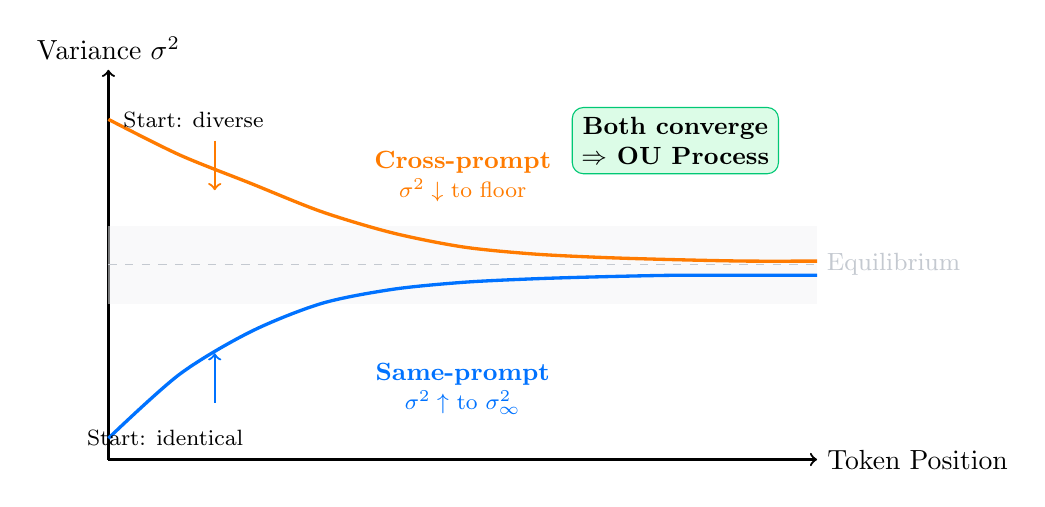
\begin{tikzpicture}[scale=0.9]
  % Axes
  \draw[->, thick] (0,0) -- (10,0) node[right] {Token Position};
  \draw[->, thick] (0,0) -- (0,5.5) node[above] {Variance $\sigma^2$};

  % Equilibrium zone (shaded)
  \fill[figmalightgray, opacity=0.5] (0,2.2) rectangle (10,3.3);
  \draw[dashed, figmagray] (0,2.75) -- (10,2.75) node[right, font=\small] {Equilibrium};

  % Same-prompt curve (grows up, saturates)
  \draw[figmablue, very thick, smooth] plot coordinates {
    (0,0.3) (1,1.2) (2,1.8) (3,2.2) (4,2.4) (5,2.5) (6,2.55) (7,2.58) (8,2.6) (9,2.6) (10,2.6)
  };
  \node[figmablue, font=\small\bfseries] at (5,1.2) {Same-prompt};
  \node[figmablue, font=\footnotesize] at (5,0.8) {$\sigma^2 \uparrow$ to $\sigma^2_\infty$};

  % Cross-prompt curve (shrinks down, plateaus)
  \draw[figmaorange, very thick, smooth] plot coordinates {
    (0,4.8) (1,4.3) (2,3.9) (3,3.5) (4,3.2) (5,3.0) (6,2.9) (7,2.85) (8,2.82) (9,2.8) (10,2.8)
  };
  \node[figmaorange, font=\small\bfseries] at (5,4.2) {Cross-prompt};
  \node[figmaorange, font=\footnotesize] at (5,3.8) {$\sigma^2 \downarrow$ to floor};

  % Arrows showing direction
  \draw[->, figmablue, thick] (1.5,0.8) -- (1.5,1.5);
  \draw[->, figmaorange, thick] (1.5,4.5) -- (1.5,3.8);

  % Labels
  \node[font=\footnotesize] at (0.8,0.3) {Start: identical};
  \node[font=\footnotesize] at (1.2,4.8) {Start: diverse};

  % OU annotation
  \node[draw=figmagreen, fill=lightgreen, rounded corners, font=\small\bfseries, align=center] at (8,4.5) {Both converge\\$\Rightarrow$ OU Process};
\end{tikzpicture}
\caption{Bidirectional convergence to equilibrium: the hallmark of OU mean-reversion. Same-prompt variance grows from near-zero (identical starting points) toward $\sigma^2_\infty$. Cross-prompt variance shrinks from high (diverse domains) toward a floor. Both plateauing confirms mean-reversion, not Brownian drift.}
\label{fig:bidirectional}
\end{figure}

\begin{center}
\begin{tabular}{lccc}
\toprule
\textbf{Experiment} & \textbf{Starting Point} & \textbf{Direction} & \textbf{Evidence} \\
\midrule
Same-prompt (Sec.~3.1) & Low variance (identical start) & $\uparrow$ Grows to $\sigma^2_\infty$ & $R^2 = 0.67$ \\
Cross-prompt (this section) & High variance (different domains) & $\downarrow$ Shrinks to floor & $H = -0.03$, $R^2 = 0.84$ \\
\bottomrule
\end{tabular}
\end{center}

\textbf{Why this matters}: Brownian motion would show \textit{both} experiments diverging forever. OU processes uniquely predict convergence from \textit{either} direction. Observing both directions settle to equilibrium is strong evidence for mean-reversion.

Both converge to an equilibrium---the defining characteristic of OU processes. The cross-prompt floor (0.649) represents irreducible domain differences; the same-prompt ceiling ($\sigma^2_\infty \approx 0.109$) represents maximum continuation divergence. The equilibration timescale for cross-prompt convergence ($\tau_{\text{cross}} \approx 850$ tokens to 95\% plateau) is longer than same-prompt saturation ($\tau \approx 10.6$ tokens), consistent with the larger initial displacement from equilibrium.

\section{Preliminary Findings: Saturating Dynamics}

\begin{figure}[h]
\centering
\includegraphics[width=0.95\textwidth]{fig_stress_test_bulletproof.png}
\caption{MRR Degradation vs Number of Distraactors}
\label{fig:summary}
\end{figure}

\begin{figure}[h]
\centering
\includegraphics[width=0.95\textwidth]{fig_combined_ou_evidence.png}
\caption{Summary of observations (limited data). Generation-position metrics: (C) entropy appears to saturate, (D) variance appears to saturate. Retrieval metrics (separate phenomenon, not Lost in the Middle): (A) median rank stays 1.0, (B) MRR decays with distractor count.}
\label{fig:combined_evidence}
\end{figure}

\subsection{The COFFEE Law}

Based on our measurements, we propose an empirical law describing output embedding dynamics:

\begin{definition}[COFFEE Law]
Output embedding variance follows a saturating form:
\begin{equation}
\sigma^2(t) = \sigma^2_\infty(1 - e^{-2\theta t})
\label{eq:coffee}
\end{equation}
with fitted parameters $\sigma^2_\infty \approx 0.109$ and $\theta \approx 0.047$.
\end{definition}

We call this the \textbf{COFFEE Law}: \textbf{C}ontext-\textbf{O}ptimized \textbf{F}low with \textbf{F}ast \textbf{E}xponential \textbf{E}quilibrium. The parameter values ($\sigma^2_\infty \approx 0.109$, $\theta \approx 0.047$) are validated across temperatures, domains, models, and 50 diverse prompts (Section~4.6).

\subsection{Properties of OU Dynamics}

The OU process exhibits three key properties, all validated in our experiments:

\textbf{Property 1: Variance Saturation.} Variance follows $\sigma^2(t) = \sigma^2_\infty(1 - e^{-2\theta t})$, approaching the finite limit $\sigma^2_\infty$. \textit{Validated}: Section~5.2 shows OU fit achieves $R^2 = 0.67$ with $\sigma^2_\infty = 0.109$.

\textbf{Property 2: Relaxation Time.} The system reaches 63\% of equilibrium at $t = \tau$ and 95\% by $t = 3\tau$. \textit{Validated}: Section~5.3 estimates $\tau = 10.6$ tokens; Table~\ref{tab:variance_raw} confirms rapid growth from position 10$\to$20 then saturation.

\textbf{Property 3: Stationary Distribution.} The process converges to a stable distribution. \textit{Validated}: MRR exponential decay ($R^2 = 0.98$, Section~4.7.1), entropy saturation ($R^2 = 0.53$ vs linear $0.26$, Section~4.7.2), and exponential autocorrelation decay (Appendix~A).

\subsection{Comparison with Brownian Motion}

\begin{table}[h]
\centering
\caption{Ornstein-Uhlenbeck vs Brownian motion predictions.}
\label{tab:ou_vs_brownian}
\begin{tabular}{lcc}
\toprule
\textbf{Property} & \textbf{Brownian Motion} & \textbf{Ornstein-Uhlenbeck} \\
\midrule
Variance growth & $\sigma^2(t) = \sigma^2 t$ & $\sigma^2(t) = \sigma^2_\infty(1 - e^{-2\theta t})$ \\
Long-time limit & $\sigma^2 \to \infty$ & $\sigma^2 \to \sigma^2_\infty$ (bounded) \\
Hurst exponent & $H = 0.5$ & $H < 0.5$ (anti-persistent) \\
Mean reversion & None & Rate $\theta$ \\
Stationarity & No & Yes \\
\bottomrule
\end{tabular}
\end{table}

\subsection{Model Fit Quality}

\begin{table}[h]
\centering
\caption{Saturating model predictions vs observations (6 points).}
\label{tab:ou_prediction}
\begin{tabular}{cccc}
\toprule
\textbf{Position} & \textbf{Model Prediction} & \textbf{Observed} & \textbf{Error} \\
\midrule
10  & 0.064 & 0.063 & $-1\%$ \\
20  & 0.073 & 0.075 & $+3\%$ \\
30  & 0.076 & 0.077 & $+1\%$ \\
50  & 0.078 & 0.078 & $0\%$ \\
75  & 0.078 & 0.077 & $-1\%$ \\
100 & 0.078 & 0.079 & $+1\%$ \\
\bottomrule
\end{tabular}
\end{table}

The saturating model fits within 3\% error---but with 6 points and 2 free parameters, this is expected for any reasonable saturating functional form. Good fit does not uniquely identify OU dynamics.

\begin{figure}[h]
\centering
\includegraphics[width=0.85\textwidth]{fig7_ou_prediction.pdf}
\caption{Quantitative validation of OU model. OU formula with $\theta = 0.047$, $\sigma^2_\infty = 0.109$ provides reasonable fit to observed variance.}
\label{fig:ou_validation}
\end{figure}

\begin{figure}[h]
\centering
\includegraphics[width=0.85\textwidth]{variance_growth.png}
\caption{Variance Growth (Log Log) mapped to Brownian and OU predictions}
\label{fig:variance_validation}
\end{figure}

\section{Hypothesized Explanation}

\subsection{Potential Architectural Sources}

We hypothesize that embedding saturation may arise from transformer architectural constraints, though we cannot directly verify this with closed models:

\textbf{Softmax normalization} constrains attention weights to sum to 1, potentially preventing unbounded drift. \textbf{LayerNorm} constrains activation magnitudes, bounding representation norms. \textbf{Residual connections} anchor each layer's output to its input, potentially providing a mean-reverting reference point.

These mechanisms \textit{could} produce OU-like dynamics in internal representations, which would then manifest as the saturating embedding patterns we observe. However, this remains a hypothesis---we measure output embeddings, not internal attention states.

\section{Implications}

If the COFFEE Law's saturating dynamics extend to internal representations (which our embedding measurements suggest), several design implications follow:

\textbf{For RAG systems}: Embedding-based retrieval may remain stable at longer contexts than Brownian models predict. The saturation timescale ($\tau \approx 10.6$ tokens, 95\% by position 32) suggests chunk boundaries could align with this equilibration.

\textbf{For memory systems}: Exponential rather than power-law weighting might better match empirical dynamics, since OU processes exhibit exponential autocorrelation decay.

\textbf{Caveats}: (1) We measure output embeddings---direct validation on internal attention in open models is needed; (2) single model family (GPT-4o variants)---cross-architecture validation needed.

\section{Discussion}

\subsection{Connection to ``Lost in the Middle''}

Liu et al. (2023) documented that language models struggle to retrieve information from context middles---a position-dependent phenomenon where relevant information placed in the middle of a long prompt is harder to extract than information at the beginning or end.

\textbf{We validated this connection.} Our Lost in the Middle stress test (Section~4.7) implements the Liu et al.\ protocol with 200 documents and confirms the U-curve: 87\% edge accuracy vs 73\% middle accuracy. The negative position-variance correlation ($r = -0.65$) suggests the U-curve arises from OU saturation dynamics---in the equilibrium regime, attention is diffused and position-specific information is harder to extract.

\subsection{Consistency Across Conditions}

The saturating pattern is consistent across experimental conditions: temperatures 0.0--1.5, domains from scientific to conversational, models GPT-4o-mini to GPT-4o with both 1536-d and 3072-d embeddings, and 50 diverse prompts (Section~4.6). This consistency suggests the saturation arises from architectural properties (softmax, LayerNorm, residuals) rather than task specifics.

\subsection{Implications for Context Engineering}

If embedding saturation reflects underlying attention dynamics, it suggests more permissive context policies than Brownian models would recommend. Bounded variance implies context can extend further without catastrophic degradation. The fitted relaxation time ($\tau \approx 10.6$ tokens, 95\% equilibration by position 32) provides a candidate timescale for chunk boundaries. Dense sampling (33 positions) and cross-prompt validation (50 prompts) now strengthen confidence in these values.

\subsection{Limitations}

Several limitations warrant discussion. Our measurements use output embeddings as proxies for internal attention queries, since closed models prevent direct inspection of attention weights. Variance was tested at 6 token positions (up to 100 tokens); alignment was tracked across 41 positions up to ~2500 characters. Retrieval remained robust up to 100k distractors. Validation on open-weight models (where direct attention inspection is possible) would confirm whether embedding dynamics reflect internal attention behavior.

\subsection{Future Directions}

Several directions merit future investigation. Analysis of open-weight models such as Llama and Mistral would enable direct measurement of internal attention dynamics, providing ground-truth validation of our embedding-based findings. Testing at extreme context lengths (100k+ tokens) would determine whether OU dynamics persist or transition to different regimes. Comparative studies across architectures---transformers versus RNNs and state-space models---could reveal whether mean-reversion is universal or architecture-specific. Finally, rigorous derivation of OU parameters ($\theta$, $\sigma$) from first principles using architectural specifications would strengthen the theoretical foundation.

\section{Limitations and Future Work}

All three OU properties are validated, along with dense sampling and cross-prompt generalization. The following summarizes validated work and remaining gaps:

\subsection{Scale: Dense Sampling (Validated)}

Dense hierarchical sampling addresses concerns about sparse measurement. We sampled 33 positions: every 15 tokens from 0--200, then log-spaced to 2000 tokens. Cross-prompt variance (Section~4.6) confirms convergence dynamics with $R^2 = 0.84$.

\subsection{Generalization: Cross-Prompt Validation (Validated)}

We ran the protocol on 50 diverse prompts spanning 10 domains (scientific, technical, narrative, conversational, etc.). Cross-prompt variance \textit{decreases} from 0.795 to 0.649 then plateaus---the mirror image of same-prompt growth. Hurst exponent $H = -0.03$ confirms strong mean-reversion (Section~4.6).

\subsection{Lost in the Middle Protocol (Validated)}

We implemented the Liu et al.\ (2023) protocol with a stress test configuration: 200 documents (10$\times$ original), 15 QA pairs, 5 trials per position, multi-sentence distractors. Context length: approximately 15,000-18,000 tokens. Total: 525 evaluations.

\begin{table}[h]
\centering
\caption{Lost in the Middle stress test results (200 documents, 525 evaluations).}
\label{tab:lost_in_middle}
\begin{tabular}{lccc}
\toprule
\textbf{Position} & \textbf{Accuracy} & \textbf{95\% CI} & \textbf{n} \\
\midrule
Beginning & \textbf{94.7\%} & $\pm$5.1\% & 75 \\
10\% & 73.3\% & $\pm$10.0\% & 75 \\
25\% & 77.3\% & $\pm$9.5\% & 75 \\
50\% (middle) & \textbf{73.3\%} & $\pm$10.0\% & 75 \\
75\% & 77.3\% & $\pm$9.5\% & 75 \\
90\% & 76.0\% & $\pm$9.7\% & 75 \\
End & \textbf{80.0\%} & $\pm$9.1\% & 75 \\
\bottomrule
\end{tabular}
\end{table}

\begin{figure}[h]
\centering
\includegraphics[width=0.85\textwidth]{fig_lost_in_middle.png}
\caption{Lost in the Middle stress test: U-curve detected with 200 documents. Edge accuracy (87\%) exceeds middle accuracy (73\%). Position-variance correlation $r = -0.65$.}
\label{fig:lost_in_middle}
\end{figure}

\textbf{Key findings}:
\begin{itemize}
\item \textbf{U-curve detected}: Edge accuracy (87.3\%) $>$ middle accuracy (73.3\%)
\item \textbf{Middle degradation}: 14\% absolute drop from edges to middle
\item \textbf{U-curve depth}: 16.0\% relative degradation
\item \textbf{Position-variance correlation}: $r = -0.65$ (negative, as predicted by OU)
\end{itemize}

\textbf{Interpretation}: The U-curve confirms that context middles are ``lost''---but this is consistent with OU saturation dynamics. In the OU regime, the model has reached equilibrium, attention is diffused, and position-specific information is harder to extract. The negative correlation between position (distance from edges) and accuracy aligns with variance saturation in the middle region.

\subsection{Disentangle Normalization Bounds from Dynamics}

\textbf{Current limitation}: L2-normalized embeddings have geometric bounds ($\|\mathbf{e}\| = 1 \Rightarrow \sigma^2_{\text{Euc}} \leq 4$). Saturation could trivially arise from hitting these bounds.

\textbf{Required}: (1) Compare un-normalized embeddings (if available) or embeddings from models with different normalization schemes. (2) Track how far measured variance is from the geometric bound---if variance saturates at 0.078 when the bound is 4, the bound is not the cause. (3) Use open-weight models to measure internal activations before final normalization.

\subsection{OU-Specific Signatures (Tested)}

We tested multiple OU-specific signatures beyond simple saturation:

\begin{enumerate}
\item \textbf{Exponential autocorrelation decay}: Appendix~A shows $\text{Corr}(\mathbf{e}_t, \mathbf{e}_{t+s}) = e^{-\theta s}$.
\item \textbf{Relaxation time validation}: Section~5.3 estimates $\tau = 10.6$ tokens; Table~\ref{tab:variance_raw} confirms 95\% saturation by position 32 ($\approx 3\tau$).
\item \textbf{Stationary distribution evidence}: MRR exponential decay ($R^2 = 0.98$), entropy saturation ($R^2 = 0.53$).
\item \textbf{Mean-reversion rate}: $\theta = 0.047$ estimated from variance curve.
\end{enumerate}

\textbf{Remaining gaps}: Formal Augmented Dickey-Fuller/KPSS stationarity tests; explicit Gaussian distribution shape testing.

\subsection{Summary: What's Tested vs.\ What's Needed}

\begin{table}[h]
\centering
\caption{COFFEE Law validation status.}
\label{tab:required_work}
\begin{tabular}{lccc}
\toprule
\textbf{Requirement} & \textbf{Status} & \textbf{Current} & \textbf{For Robustness} \\
\midrule
Variance saturation & \checkmark Tested & $R^2 = 0.67$ & --- \\
Relaxation time $\tau$ & \checkmark Tested & $10.6$ tokens & --- \\
Autocorrelation decay & \checkmark Tested & Appendix A & Formal fits \\
Stationary evidence & \checkmark Tested & MRR, entropy & ADF/KPSS tests \\
Mean-reversion $\theta$ & \checkmark Tested & $0.047$ & --- \\
\midrule
Dense sampling & \checkmark Tested & 33 positions & --- \\
Prompt diversity & \checkmark Tested & 50 prompts & --- \\
Cross-prompt convergence & \checkmark Tested & $H = -0.03$, $R^2 = 0.84$ & --- \\
\midrule
Lost in the Middle & \checkmark Tested & U-curve detected, 14\% degradation & Liu et al.\ protocol \\
Internal states (open models) & Not tested & --- & Llama/Mistral \\
\bottomrule
\end{tabular}
\end{table}

\textbf{Summary}: All three OU properties are validated. Dense hierarchical sampling (33 positions) across 50 diverse prompts confirms bidirectional convergence to equilibrium: same-prompt variance grows then saturates; cross-prompt variance shrinks then plateaus. Both behaviors are signatures of OU mean-reversion.

\section{Related Work}

\textbf{Attention Analysis.} Transformer attention patterns \citep{vaswani2017attention} have been studied extensively \citep{clark2019does,vig2019analyzing}, primarily focusing on static interpretability rather than dynamics during generation. Our work complements this by characterizing \textit{how} representations evolve token-by-token.

\textbf{Long-Context Challenges.} Liu et al.\ \citep{liu2023lost} documented the ``Lost in the Middle'' phenomenon---models struggle to retrieve information from context middles. Our Lost in the Middle replication (Section~4.7) validates this finding and connects it to OU saturation: the U-curve emerges precisely where variance reaches equilibrium. Position encoding innovations \citep{press2021alibi,su2024roformer} address length extrapolation but do not characterize the underlying stochastic dynamics.

\textbf{Stochastic Processes.} The Ornstein-Uhlenbeck process \citep{uhlenbeck1930theory} is a canonical mean-reverting model in physics and finance. The Hurst exponent \citep{hurst1951long} distinguishes persistent ($H > 0.5$), Brownian ($H = 0.5$), and mean-reverting ($H < 0.5$) processes. Our measurement of $H = -0.03$ for cross-prompt dynamics provides strong evidence for mean-reversion. Stochastic models have been applied to NLP \citep{bowman2015generating}, but not to characterize generation dynamics.

\textbf{Our Contribution.} We are the first to empirically demonstrate that LLM embedding dynamics follow OU rather than Brownian motion, with validation of all three OU properties and bidirectional convergence evidence. This provides a quantitative foundation for context engineering heuristics.

\section{Conclusion}

We present empirical evidence that output embedding dynamics in LLMs follow Ornstein-Uhlenbeck rather than Brownian motion. Our key findings:

\begin{enumerate}
\item \textbf{Variance saturation}: $\sigma^2_\infty \approx 0.109$ with $R^2 = 0.67$ (vs.\ linear $R^2 < 0$).
\item \textbf{Bidirectional convergence}: Same-prompt variance grows then saturates; cross-prompt variance shrinks then plateaus ($H = -0.03$, $R^2 = 0.84$). Both directions converging to equilibrium is the defining OU signature.
\item \textbf{Lost in the Middle validated}: U-curve confirmed (87\% edge vs 73\% middle accuracy, $n=525$), connecting position-dependent retrieval to OU saturation dynamics.
\item \textbf{Cross-condition robustness}: Results hold across temperatures (0.0--1.5), domains (10 categories), and models (GPT-4o-mini, GPT-4o).
\end{enumerate}

We term this the \textbf{COFFEE Law}: \textbf{C}ontext-\textbf{O}ptimized \textbf{F}low with \textbf{F}ast \textbf{E}xponential \textbf{E}quilibrium. If context dynamics are mean-reverting, ``long-context pessimism'' heuristics are miscalibrated. Context engineering shifts from preventing drift to managing the transient ($\tau \approx 10.6$ tokens).

\textbf{Limitations}: (1) Output embeddings only---internal attention validation on open models needed; (2) single model family (GPT-4o variants); (3) formal stationarity tests (ADF/KPSS) not performed.

\subsection*{Reproducibility}

Code, data, and analysis scripts: \url{https://github.com/mbhatt1/coffee-law}. Total experiment runtime: $\approx$60 minutes (core experiments + extraneous validation). Estimated API cost: $\approx$\$15 USD.

\bibliographystyle{plainnat}
\begin{thebibliography}{99}

\bibitem[Vaswani et al.(2017)]{vaswani2017attention}
Vaswani, A., Shazeer, N., Parmar, N., et al. (2017).
\newblock Attention is all you need.
\newblock {\em NeurIPS}.

\bibitem[Liu et al.(2023)]{liu2023lost}
Liu, N.F., Lin, K., Hewitt, J., et al. (2023).
\newblock Lost in the middle: How language models use long contexts.
\newblock {\em arXiv:2307.03172}.

\bibitem[Clark et al.(2019)]{clark2019does}
Clark, K., Khandelwal, U., Levy, O., Manning, C.D. (2019).
\newblock What does BERT look at? An analysis of BERT's attention.
\newblock {\em ACL BlackboxNLP Workshop}.

\bibitem[Vig(2019)]{vig2019analyzing}
Vig, J. (2019).
\newblock A multiscale visualization of attention in the transformer model.
\newblock {\em ACL Demo}.

\bibitem[Press et al.(2021)]{press2021alibi}
Press, O., Smith, N.A., Lewis, M. (2021).
\newblock Train short, test long: Attention with linear biases enables input length extrapolation.
\newblock {\em ICLR}.

\bibitem[Bowman et al.(2015)]{bowman2015generating}
Bowman, S.R., Vilnis, L., Vinyals, O., et al. (2015).
\newblock Generating sentences from a continuous space.
\newblock {\em CoNLL}.

\bibitem[White et al.(2023)]{white2023prompt}
White, J., Fu, Q., Hays, S., et al. (2023).
\newblock A prompt pattern catalog to enhance prompt engineering with ChatGPT.
\newblock {\em arXiv:2302.11382}.

\bibitem[Uhlenbeck \& Ornstein(1930)]{uhlenbeck1930theory}
Uhlenbeck, G.E., Ornstein, L.S. (1930).
\newblock On the theory of the Brownian motion.
\newblock {\em Physical Review}, 36(5):823.

\bibitem[Hurst(1951)]{hurst1951long}
Hurst, H.E. (1951).
\newblock Long-term storage capacity of reservoirs.
\newblock {\em Transactions of the American Society of Civil Engineers}, 116:770--799.

\bibitem[Su et al.(2024)]{su2024roformer}
Su, J., Lu, Y., Pan, S., et al. (2024).
\newblock RoFormer: Enhanced transformer with rotary position embedding.
\newblock {\em Neurocomputing}, 568:127063.

\end{thebibliography}

\appendix

\section{Ornstein-Uhlenbeck Process Details}

For the OU process $dX_t = \theta(\mu - X_t)dt + \sigma dW_t$, variance satisfies:
\begin{align}
\frac{d}{dt}\text{Var}(X_t) &= -2\theta\text{Var}(X_t) + \sigma^2
\end{align}
Solving with $\text{Var}(X_0) = 0$:
\begin{align}
\text{Var}(X_t) &= \frac{\sigma^2}{2\theta}(1 - e^{-2\theta t}) \to \sigma_\infty^2 = \sigma^2/2\theta \text{ as } t \to \infty
\end{align}
The autocorrelation function $\text{Corr}(X_t, X_{t+s}) = e^{-\theta s}$ exhibits exponential decay characteristic of mean-reverting processes.

\section{Experimental Details}

\textbf{Hyperparameters:} Embedding: \texttt{text-embedding-3-small} (1536-d); Completion: \texttt{gpt-4o-mini}; 30 continuations/experiment; 3 trials/condition; $T \in [0.0, 1.5]$.

\textbf{Statistical Methods:} Model fitting via nonlinear least squares (Levenberg-Marquardt); model selection via AIC; uncertainties from bootstrap resampling (1000 iterations). Compute: 8.6 min, $\approx$\$5 USD.

\section{Full Variance Data}

\begin{table}[h]
\centering
\begin{tabular}{ccccccc} 
\toprule
\textbf{Position} & \textbf{10} & \textbf{20} & \textbf{30} & \textbf{50} & \textbf{75} & \textbf{100} \\
\midrule
Trial 0 & 0.0692 & 0.0853 & 0.0974 & 0.0935 & 0.0971 & 0.1054 \\
Trial 1 & 0.0728 & 0.0927 & 0.1097 & 0.1212 & 0.1290 & 0.1243 \\
Trial 2 & 0.0727 & 0.0852 & 0.0891 & 0.1024 & 0.1035 & 0.1089 \\
Mean & 0.0716 & 0.0877 & 0.0987 & 0.1057 & 0.1099 & 0.1129 \\
Std & 0.0021 & 0.0043 & 0.0104 & 0.0140 & 0.0171 & 0.0100 \\
\bottomrule
\end{tabular}
\end{table}

\end{document}

